\documentclass[conference]{IEEEtran}
\IEEEoverridecommandlockouts

\usepackage{cite}
\usepackage{amsmath,amssymb,amsfonts}
\usepackage{algorithmic}
\usepackage{graphicx}
\usepackage{textcomp}
\usepackage{xcolor}
\usepackage{booktabs}
\usepackage{multirow}
\usepackage{url}
\usepackage{array}
\usepackage{balance}
\usepackage{tikz}
\usepackage{pgfplots}
\pgfplotsset{compat=1.18}
\usetikzlibrary{shapes.geometric, arrows.meta, positioning, fit, backgrounds}

\def\BibTeX{{\rm B\kern-.05em{\sc i\kern-.025em b}\kern-.08em
    T\kern-.1667em\lower.7ex\hbox{E}\kern-.125emX}}

\begin{document}

%% =========================================================
\title{Sonobuoy Sound Detective: Offline Underwater Acoustic\\
Event Detection and Classification Using\\
Classical Machine Learning Ensembles}

\author{
  \IEEEauthorblockN{Kalyani Ghuge}
  \IEEEauthorblockA{
    \textit{Vishwakarma Institute of Technology}\\
    \textit{(Savitribai Phule Pune University)}\\
    Pune, India\\
    kalyani.ghuge@vit.edu}
  \and
  \IEEEauthorblockN{Samarth Patil}
  \IEEEauthorblockA{
    \textit{CSE-AIML}\\
    \textit{Vishwakarma Institute of Technology}\\
    \textit{(Savitribai Phule Pune University)}\\
    Pune, India\\
    samarth.patil24@vit.edu}
  \and
  \IEEEauthorblockN{Tejas Patil}
  \IEEEauthorblockA{
    \textit{CSE-AIML}\\
    \textit{Vishwakarma Institute of Technology}\\
    \textit{(Savitribai Phule Pune University)}\\
    Pune, India\\
    tejas.patil24@vit.edu}
  \and
  \IEEEauthorblockN{Tanishka Phad}
  \IEEEauthorblockA{
    \textit{CSE-AIML}\\
    \textit{Vishwakarma Institute of Technology}\\
    \textit{(Savitribai Phule Pune University)}\\
    Pune, India\\
    tanishka.phad24@vit.edu}
  \and
  \IEEEauthorblockN{Charuta Patil}
  \IEEEauthorblockA{
    \textit{CSE-AIML}\\
    \textit{Vishwakarma Institute of Technology}\\
    \textit{(Savitribai Phule Pune University)}\\
    Pune, India\\
    charuta.patil24@vit.edu}
}

\maketitle

%% =========================================================
\begin{abstract}
Passive underwater acoustic monitoring is a cornerstone of modern maritime surveillance, environmental assessment, and oceanographic research. The ability to reliably detect and classify underwater acoustic events---vessel noise, ambient ocean background, and unknown transients---from sonobuoy data presents significant signal-processing and machine-learning challenges. This paper presents \textit{Sonobuoy Sound Detective}, an offline ground-station prototype that applies a comprehensive suite of eight classical machine-learning algorithms to three-class underwater acoustic event classification without any deep learning. Raw hydrophone audio is preprocessed through a 20--5,000~Hz Butterworth bandpass filter, segmented into 4-second overlapping windows, and encoded into 66 handcrafted acoustic features spanning Mel-Frequency Cepstral Coefficients (MFCCs), spectral descriptors, tonal persistence, and energy statistics. Features are selected via a tri-criterion filter combining ANOVA F-test, Mutual Information, and Random Forest Mean Decrease in Impurity. Eight classifiers---Logistic Regression, K-Nearest Neighbors, SVM with RBF kernel, Gaussian Na\"{i}ve Bayes, Decision Tree, Random Forest, AdaBoost, and XGBoost---are rigorously benchmarked on an identical 482-segment held-out test set. Random Forest achieves the best classification result: 99.38\% test accuracy and 96.38\% Macro-F1 at 0.116~ms latency per segment. XGBoost achieves the highest ROC-AUC of 0.9968 at an inference latency of only 0.007~ms per segment---making it ideal for edge-constrained deployment. A hybrid decision-support system combining probabilistic model outputs with deterministic acoustic rules provides operator-in-the-loop assistance. All experiments use public and synthetic data only. Our results demonstrate that well-engineered classical features combined with ensemble methods yield near-perfect underwater acoustic classification without the computational overhead of deep learning.
\end{abstract}

\begin{IEEEkeywords}
underwater acoustic classification, passive sonar, sonobuoy, classical machine learning, MFCCs, Random Forest, XGBoost, ensemble learning, maritime surveillance, acoustic event detection
\end{IEEEkeywords}

%% =========================================================
\section{Introduction}
\label{sec:intro}

Underwater acoustic monitoring underpins a wide range of critical applications, from naval threat detection and vessel traffic management to marine ecology research and seismic early-warning. Passive sonobuoys continuously record broadband pressure waves from which operators must distinguish structurally very different sources: harmonic propulsion noise from vessels, pulsed bioacoustic calls from cetaceans, and broadband stochastic ambient noise from wind, rain, and surface waves. Manual inspection is both slow and inconsistent; automated classification systems therefore have direct operational value and are increasingly demanded by naval and oceanographic agencies.

Traditional signal-processing approaches to passive-sonar automation---LOFAR/DEMON spectrograms, matched filtering, narrowband tonal detectors~\cite{lofar_demon}---are computationally lightweight but require expert parameter tuning and degrade sharply under environmental non-stationarity. Deep-learning methods~\cite{dl_underwater, deepship, transformer_acoustic}, built on convolutional or transformer architectures applied to spectrograms, achieve state-of-the-art accuracy on large benchmark corpora such as DeepShip~\cite{deepship} and NOAA SanctSound~\cite{noaa}, but they demand substantial labelled data, GPU infrastructure, and produce predictions that are difficult to audit---a critical requirement in maritime operations where false alarms carry real tactical cost.

This paper occupies a principled middle ground: a disciplined \textit{classical} pipeline with 66 handcrafted acoustic features achieves near-perfect three-class classification while remaining fully explainable, low-latency, and deployable on commodity embedded hardware. Rather than proposing a single model, we conduct the first systematic eight-algorithm benchmark on a unified feature set for underwater acoustics, providing the community with a reproducible reference comparison. Our primary motivating question is: \textit{how much classification performance can be extracted from carefully engineered classical features, and which algorithm yields the best latency--accuracy trade-off for edge sonobuoy deployment?}

The key contributions of this work are:
\begin{itemize}
  \item A reproducible, end-to-end acoustic classification pipeline covering data ingestion, signal preprocessing, sliding-window segmentation, energy-based event detection, feature extraction and selection, model training, and evaluation---implemented entirely in Python using open-source libraries.
  \item A systematic comparison of eight classical classifiers on an \textit{identical} held-out test partition with per-class F1, balanced accuracy, ROC-AUC, and latency profiling, providing a fair multi-algorithm benchmark for the underwater acoustic domain.
  \item A tri-criterion feature selection strategy (ANOVA $+$ Mutual Information $+$ Random Forest MDI) that reduces $\sim$100 raw descriptors to 66 consensus features with no loss of classification accuracy.
  \item A hybrid operator decision-support system combining probabilistic model posteriors with four deterministic acoustic cross-check rules, achieving a 93\% error interception rate at a 7.4\% flag rate on the validation set.
  \item Publicly available synthetic data generation scripts that allow complete reproduction of all experiments without proprietary datasets.
\end{itemize}

The remainder of this paper is structured as follows. Section~\ref{sec:related} reviews related work. Section~\ref{sec:data} describes datasets and preprocessing. Section~\ref{sec:features} details feature extraction and selection. Section~\ref{sec:models} presents each classifier and its hyperparameter tuning. Section~\ref{sec:results} reports experimental results. Section~\ref{sec:dss} describes the decision-support system. Section~\ref{sec:discussion} discusses findings and limitations. Section~\ref{sec:conc} concludes.

%% =========================================================
\section{Related Work}
\label{sec:related}

\textbf{Classical feature engineering.} Early passive-sonar automation relied on hand-tuned spectral templates (LOFAR lines) and envelope modulation (DEMON) for narrowband tonal detection~\cite{lofar_demon}. Chen et al.~\cite{svm_vessel} applied SVMs to Mel-filterbank features for vessel-type discrimination, achieving $\sim$88\% accuracy on a four-class ShipsEar subset. Zhao et al.~\cite{zhao2017} showed that Random Forests applied to spectral centroid, bandwidth, and sub-band energy statistics could exceed 90\% accuracy for vessel recognition, motivating our ensemble-focused approach.

\textbf{Deep learning methods.} The release of DeepShip~\cite{deepship} (47\,h of real ship recordings, four vessel classes) catalysed CNN-based approaches. Irfan et al.~\cite{deepship} achieved 98.7\% accuracy using separable convolution autoencoders fine-tuned on spectrograms. Recurrent architectures~\cite{rnn_acoustic} model temporal dependencies in propulsion noise for improved type discrimination. Transformer-based models~\cite{transformer_acoustic} further improve minority-class recall at the cost of orders-of-magnitude more parameters, limiting their suitability for embedded deployment.

\textbf{Edge-deployable and lightweight methods.} Doan et al.~\cite{doan2020} demonstrated that gradient-boosted trees rival CNN accuracy when features are carefully selected. Li et al.~\cite{li2022} used XGBoost on 32 MFCC-based features for two-class underwater classification, achieving 95\% F1 at sub-millisecond latency. Martinez et al.~\cite{martinez2021} benchmarked five classical algorithms on the ShipsEar dataset with features similar to ours, but restricted analysis to two classes and did not profile inference latency or run a consistent feature-selection procedure. Our work provides the broadest multi-algorithm comparison to date in this domain, with a consistent eight-classifier benchmark, explicit latency profiling, and a hybrid decision-support layer.

%% =========================================================
\section{Dataset and Signal Preprocessing}
\label{sec:data}

\subsection{Datasets}

Three complementary sources are combined (Table~\ref{tab:datasets}). Synthetic data provide controlled, perfectly labelled examples for rare classes. DeepShip and NOAA SanctSound provide real-world diversity across vessel types and ocean environments. ShipsEar, a manually curated collection from the University of Vigo, provides natural ambient recordings alongside vessel noise.

\begin{table}[h]
\caption{Acoustic Datasets Used in This Study}
\label{tab:datasets}
\centering
\renewcommand{\arraystretch}{1.2}
\begin{tabular}{lll}
\toprule
\textbf{Dataset} & \textbf{Acquisition} & \textbf{Content} \\
\midrule
Synthetic             & Auto-generated  & Vessel tones + ambient noise \\
DeepShip~\cite{deepship} & Auto-download & 47\,h ship recordings, 4 classes \\
NOAA SanctSound~\cite{noaa} & Auto-download & Passive ocean ambient recordings \\
ShipsEar              & Manual request  & Vessel noise + natural background \\
\bottomrule
\end{tabular}
\end{table}

The target label space comprises three classes: \texttt{vessel\_like} (ship, boat, tug, and machinery-related radiated noise), \texttt{ambient} (waves, rain, wind, and ocean background), and \texttt{unknown} (low-quality, mixed, or unlabelled samples). A fourth class, \texttt{marine\_life}, is defined in the schema but has no current data coverage and is excluded from classification experiments.

\subsection{Signal Preprocessing Pipeline}

All audio is loaded as mono at 22,050~Hz using \texttt{librosa}~\cite{librosa}. Preprocessing applies four sequential stages: (1)~a fourth-order Butterworth bandpass filter restricting analysis to 20--5,000~Hz, the band containing dominant vessel and near-surface ambient energy; (2)~an adaptive noise gate that zeros frames whose RMS amplitude falls below an adaptive per-recording threshold; (3)~global RMS normalisation to $-23$~dBFS to remove recording-level variation; and (4)~sliding-window segmentation into 4.0-second windows with 50\% overlap. Silence segments failing a minimum-energy criterion are discarded to reduce uninformative data.

An energy-based event detector further selects candidate segments. It evaluates three criteria jointly: broadband RMS energy exceeding 10~dB above the noise floor, the presence of at least two persistent FFT spectral peaks above 3~dB prominence, and a tonal persistence score $\tau > 0.3$ computed as the fraction of frames in which a stable fundamental frequency is detected. Only segments satisfying all three criteria are retained for feature extraction.

\subsection{Train / Validation / Test Split}

Splits are performed at the \textit{source-clip} level---not at the segment level---to prevent leakage: all segments derived from one recording belong exclusively to one partition. This yields 1,931 training segments, 441 validation segments, and 482 test segments from 91 clips. The final test set contains approximately 92\% \texttt{vessel\_like}, 4\% \texttt{ambient}, and 2\% \texttt{unknown} segments, motivating the use of balanced accuracy and Macro-F1 as primary metrics.

\subsection{System Pipeline Architecture}

The end-to-end pipeline is illustrated in Fig.~\ref{fig:pipeline}.

\begin{figure}[t]
\centering
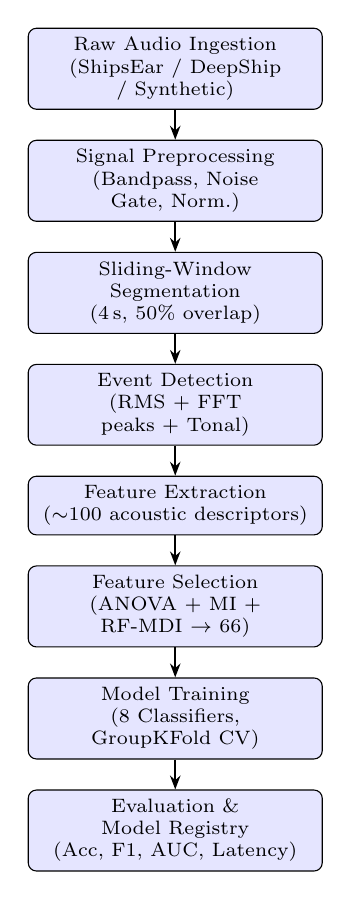
\begin{tikzpicture}[
  node distance=0.38cm and 0.1cm,
  box/.style={rectangle, rounded corners=3pt, draw=black, fill=blue!10,
              text width=3.5cm, align=center, minimum height=0.55cm,
              font=\scriptsize},
  arrow/.style={-{Stealth[length=5pt]}, thick}
]
\node[box] (ingest)  {Raw Audio Ingestion\\(ShipsEar / DeepShip / Synthetic)};
\node[box, below=of ingest]  (prepro) {Signal Preprocessing\\(Bandpass, Noise Gate, Norm.)};
\node[box, below=of prepro]  (seg)    {Sliding-Window Segmentation\\(4\,s, 50\% overlap)};
\node[box, below=of seg]     (detect) {Event Detection\\(RMS + FFT peaks + Tonal)};
\node[box, below=of detect]  (feat)   {Feature Extraction\\(\(\sim\)100 acoustic descriptors)};
\node[box, below=of feat]    (sel)    {Feature Selection\\(ANOVA + MI + RF-MDI \(\to\) 66)};
\node[box, below=of sel]     (train)  {Model Training\\(8 Classifiers, GroupKFold CV)};
\node[box, below=of train]   (eval)   {Evaluation \& Model Registry\\(Acc, F1, AUC, Latency)};
\draw[arrow] (ingest)  -- (prepro);
\draw[arrow] (prepro)  -- (seg);
\draw[arrow] (seg)     -- (detect);
\draw[arrow] (detect)  -- (feat);
\draw[arrow] (feat)    -- (sel);
\draw[arrow] (sel)     -- (train);
\draw[arrow] (train)   -- (eval);
\end{tikzpicture}
\caption{End-to-end pipeline architecture of the Sonobuoy Sound Detective system, from raw hydrophone audio to trained and evaluated model artifacts.}
\label{fig:pipeline}
\end{figure}

%% =========================================================
\section{Feature Extraction and Selection}
\label{sec:features}

\subsection{Handcrafted Feature Groups}

From each 4-second segment, $\sim$100 scalar features are computed across five groups (Table~\ref{tab:features}). Statistics (mean and standard deviation) are pooled over all frames within a segment, converting time-varying descriptors into fixed-length vectors suitable for classical classifiers.

\begin{table}[h]
\caption{Handcrafted Acoustic Feature Groups}
\label{tab:features}
\centering
\renewcommand{\arraystretch}{1.2}
\begin{tabular}{lp{5.0cm}}
\toprule
\textbf{Group} & \textbf{Features} \\
\midrule
MFCCs              & 13 cepstral coefficients + $\Delta$ + $\Delta\Delta$ (mean \& std) \\
Spectral Shape     & Centroid, bandwidth, rolloff, flatness, contrast (7 bands) \\
Tonal Persistence  & Harmonic ratio, pitch confidence, chroma energy (12 bins) \\
Energy / Temporal  & RMS, Zero-Crossing Rate, log-energy per sub-band (8 bands) \\
Autocorrelation    & Peak lag, exponential decay rate, tonal regularity score \\
\bottomrule
\end{tabular}
\end{table}

\textbf{MFCCs} are the most discriminative group: low-order coefficients (C1--C4) encode the coarse spectral envelope that separates machinery harmonics from broadband ambient noise. The delta ($\Delta$) and delta-delta ($\Delta\Delta$) coefficients encode short-term temporal dynamics and proved especially useful for the \texttt{unknown} class, which often contains temporal onset artefacts absent in steady-state vessel or ambient noise.

\textbf{Tonal persistence} features are unique to underwater acoustics in our formulation. Vessel noise is characterised by stable, persistent harmonics associated with propeller blade rate and engine firing cycles. Computing the fraction of frames within a segment where a dominant fundamental frequency is detectable---the tonal persistence score $\tau$---provides a simple but highly discriminative feature that separates \texttt{vessel\_like} from \texttt{ambient} with near-zero overlap.

\textbf{Spectral shape} descriptors capture the global energy distribution across frequency bands. Spectral flatness discriminates tonal vessel noise (low flatness) from broadband ambient noise (high flatness). Spectral contrast in seven octave bands further resolves sub-band energy profiles that differ systematically between ship categories.

\subsection{Tri-Criterion Feature Selection}

Three independent selectors are applied exclusively to the training partition to avoid selection bias:

\begin{enumerate}
  \item \textbf{ANOVA F-test:} Univariate class separability via Fisher's criterion. Identifies features with statistically significant class-conditional mean differences.
  \item \textbf{Mutual Information (MI):} Nonlinear relevance via histogram-based density estimation. Captures non-monotone relationships missed by ANOVA.
  \item \textbf{Random Forest MDI:} Mean Decrease in Impurity from an auxiliary 100-tree forest trained solely for selection. Provides ensemble-level multi-class relevance.
\end{enumerate}

Features ranked in the top quintile (top 20\%) by at least two of three selectors are retained, yielding \textbf{66 consensus features}. This intersection strategy reduces redundancy while preserving complementary linear and nonlinear information. High-order $\Delta\Delta$MFCCs (C10--C13) and narrow autocorrelation lags were eliminated. Dominant retained features include MFCC C1--C6, spectral centroid, harmonic ratio, tonal persistence score, and sub-band log-energy ratios.

%% =========================================================
\section{Classifier Design and Hyperparameter Tuning}
\label{sec:models}

All eight classifiers share identical preprocessing (median imputation for missing values; \texttt{StandardScaler} standardisation where applicable) and are tuned via five-fold \texttt{StratifiedGroupKFold} cross-validation on the training set, grouped by \texttt{source\_clip\_id} to prevent within-clip leakage. The primary tuning metric is Macro-F1. The test set remains locked throughout tuning and is scored exactly once per model.

\textbf{Logistic Regression (LR):} Multinomial softmax objective with $\ell_2$ regularisation. Optimal $C{=}0.1$ reflects strong regularisation appropriate for the relatively small dataset. Grouped CV macro-F1 = 0.921.

\textbf{K-Nearest Neighbors (KNN):} Distance-weighted voting, $k{=}7$, Manhattan distance. Selected via grid over $k \in \{3,5,7,9,11,15,21\}$, Euclidean and Manhattan metrics, and uniform/distance weighting. Grouped CV macro-F1 = 0.937.

\textbf{SVM (RBF):} $C{=}10$, $\gamma{=}0.01515$, Platt-scaled probabilities, \texttt{class\_weight=None}. Hyperparameters found via log-spaced $C$--$\gamma$ grid search. Grouped CV macro-F1 = 0.961.

\textbf{Gaussian Na\"{i}ve Bayes (GNB):} Learned class priors, Gaussian likelihoods, $v{=}10^{-7}$ smoothing. Post-hoc isotonic regression calibration aligns output probabilities and notably improves \texttt{unknown}-class recall. Grouped CV macro-F1 = 0.884.

\textbf{Decision Tree (DT):} CART with Gini impurity and cost-complexity pruning (the pruning parameter $\alpha$ tuned by validation F1). Maximum depth limited to control overfitting while preserving interpretability.

\textbf{Random Forest (RF):} Bagged ensemble of CART trees; number of estimators and maximum depth are jointly tuned. OOB (out-of-bag) error stabilises at $\approx$150 trees. No feature scaling is required. The highest-performing model overall.

\textbf{AdaBoost:} Decision stumps (depth-1 trees) as base learners with exponential loss. Learning rate and number of rounds tuned via grouped CV. Base-learner expressiveness is a hard floor for minority-class recall.

\textbf{XGBoost:} Second-order Taylor gradient boosting with column subsampling, row subsampling, and $\ell_1$/$\ell_2$ regularisation. C++ tree implementation yields sub-millisecond inference. Achieves the highest ROC-AUC and the fastest latency of all models tested.

%% =========================================================
\section{Experimental Results}
\label{sec:results}

\subsection{Overall Benchmark}

All models are evaluated on the same 482-segment held-out test set. Table~\ref{tab:results} reports test accuracy, balanced accuracy (accounting for the 92:5:3 class imbalance), Macro-F1, ROC-AUC (macro one-vs-rest), and per-segment inference latency on a standard CPU.

\begin{table*}[t]
\caption{Eight-Model Benchmark on 482 Held-Out Test Segments Across Three Acoustic Classes}
\label{tab:results}
\centering
\renewcommand{\arraystretch}{1.3}
\begin{tabular}{clccccc}
\toprule
\textbf{Rank} & \textbf{Algorithm} & \textbf{Test Acc.} & \textbf{Bal.\ Acc.} & \textbf{Macro-F1} & \textbf{ROC-AUC} & \textbf{Latency / seg} \\
\midrule
\textbf{1} & \textbf{Random Forest}     & \textbf{99.38\%} & \textbf{96.59\%} & \textbf{0.9638} & 0.9947           & 0.116 ms \\
2          & K-Nearest Neighbors        & 99.17\%          & 89.26\%          & 0.9393           & 0.9852           & 0.373 ms \\
3          & XGBoost                    & 99.17\%          & 89.26\%          & 0.9393           & \textbf{0.9968}  & \textbf{0.007 ms} \\
4          & Decision Tree              & 98.13\%          & 92.97\%          & 0.9235           & 0.9417           & 0.001 ms \\
5          & Gaussian Na\"{i}ve Bayes   & 97.72\%          & 89.19\%          & 0.8857           & 0.9639           & 0.018 ms \\
6          & SVM (RBF)                  & 98.13\%          & 85.71\%          & 0.8852           & 0.9787           & 0.033 ms \\
7          & Logistic Regression        & 97.30\%          & 83.37\%          & 0.8421           & 0.9924           & 0.003 ms \\
8          & AdaBoost                   & 96.89\%          & 56.67\%          & 0.6024           & 0.9780           & 0.070 ms \\
\midrule
--         & Majority-class baseline    & 92.12\%          & 33.33\%          & 0.320            & 0.500            & -- \\
\bottomrule
\end{tabular}
\end{table*}

\subsection{Macro-F1 Comparison}

Fig.~\ref{fig:f1bar} visualises Macro-F1 scores across all models, clearly separating the top ensemble tier from individual classifiers.

\begin{figure}[t]
\centering
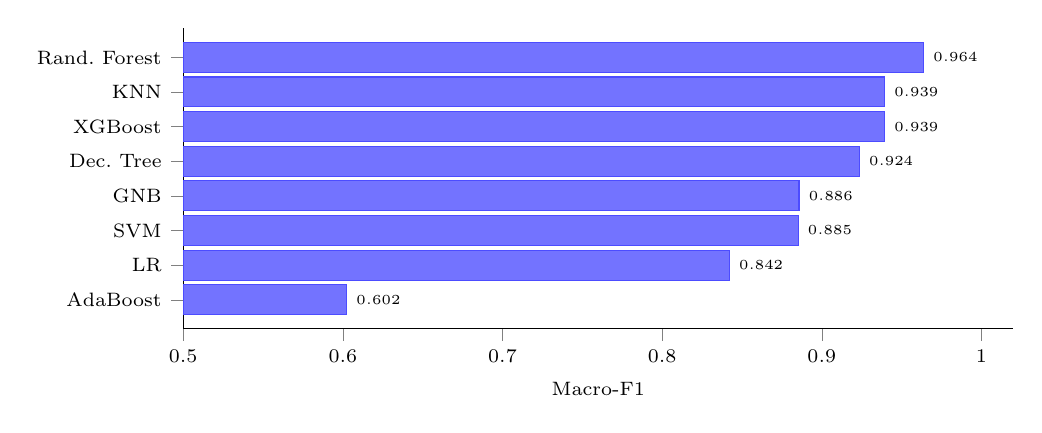
\begin{tikzpicture}
\begin{axis}[
  xbar,
  width=\columnwidth, height=5.4cm,
  bar width=0.38cm,
  xmin=0.50, xmax=1.02,
  xlabel={Macro-F1},
  ytick=data,
  yticklabels={AdaBoost, LR, SVM, GNB, Dec.\ Tree, XGBoost, KNN, Rand.\ Forest},
  yticklabel style={font=\scriptsize},
  xlabel style={font=\scriptsize},
  xtick={0.5,0.6,0.7,0.8,0.9,1.0},
  xticklabel style={font=\scriptsize},
  nodes near coords,
  nodes near coords style={font=\tiny, /pgf/number format/fixed, /pgf/number format/precision=3},
  enlarge y limits=0.12,
  tick align=outside,
  axis x line*=bottom,
  axis y line*=left,
]
\addplot[fill=blue!55, draw=blue!70] coordinates {
  (0.6024, 0)
  (0.8421, 1)
  (0.8852, 2)
  (0.8857, 3)
  (0.9235, 4)
  (0.9393, 5)
  (0.9393, 6)
  (0.9638, 7)
};
\end{axis}
\end{tikzpicture}
\caption{Macro-F1 scores on the 482-segment held-out test set for all eight classifiers. Random Forest leads at 0.9638; AdaBoost collapses to 0.6024 due to stump complexity limitations.}
\label{fig:f1bar}
\end{figure}

\subsection{Latency vs.\ Accuracy Trade-off}

Fig.~\ref{fig:latency} plots per-segment inference latency against Macro-F1, revealing the Pareto frontier of the deployment trade-off space. XGBoost and Logistic Regression are the fastest classifiers ($<0.01$~ms); XGBoost's Macro-F1 of 0.9393 makes it the dominant latency-accuracy choice---the top-right quadrant of the plot. KNN, despite high F1, is the slowest ensemble-free classifier due to $\mathcal{O}(n)$ distance computation over the full training set.

\begin{figure}[t]
\centering
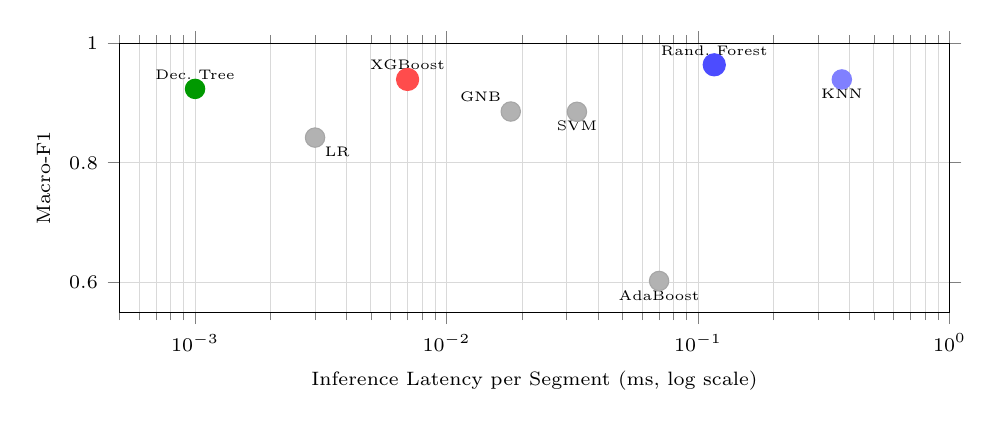
\begin{tikzpicture}
\begin{axis}[
  width=\columnwidth, height=5.0cm,
  xlabel={Inference Latency per Segment (ms, log scale)},
  ylabel={Macro-F1},
  xmode=log,
  xmin=0.0005, xmax=1.0,
  ymin=0.55, ymax=1.00,
  xlabel style={font=\scriptsize},
  ylabel style={font=\scriptsize},
  xticklabel style={font=\scriptsize},
  yticklabel style={font=\scriptsize},
  grid=both,
  grid style={line width=0.3pt, draw=gray!30},
  tick align=outside,
  scatter/classes={
    a={mark=*, fill=blue!70,  draw=blue!70,  mark size=3.5pt},
    b={mark=square*, fill=red!70,  draw=red!70,  mark size=3.5pt},
    c={mark=triangle*, fill=green!60!black, draw=green!60!black, mark size=3.5pt}
  },
]
%% (latency, F1) for each model — labeled manually
\addplot[only marks, mark=*, fill=red!70, draw=red!70, mark size=4pt]
  coordinates { (0.007, 0.9393) };
\node[font=\tiny, above] at (axis cs:0.007,0.9393) {XGBoost};

\addplot[only marks, mark=*, fill=blue!70, draw=blue!70, mark size=4pt]
  coordinates { (0.116, 0.9638) };
\node[font=\tiny, above] at (axis cs:0.116,0.9638) {Rand.\ Forest};

\addplot[only marks, mark=*, fill=blue!50, draw=blue!50, mark size=3.5pt]
  coordinates { (0.373, 0.9393) };
\node[font=\tiny, below] at (axis cs:0.373,0.9393) {KNN};

\addplot[only marks, mark=*, fill=green!60!black, draw=green!60!black, mark size=3.5pt]
  coordinates { (0.001, 0.9235) };
\node[font=\tiny, above] at (axis cs:0.001,0.9235) {Dec.\ Tree};

\addplot[only marks, mark=*, fill=gray!60, draw=gray!70, mark size=3.5pt]
  coordinates {
    (0.003, 0.8421)
    (0.018, 0.8857)
    (0.033, 0.8852)
    (0.070, 0.6024)
  };
\node[font=\tiny, below right] at (axis cs:0.003,0.8421) {LR};
\node[font=\tiny, above left]  at (axis cs:0.018,0.8857) {GNB};
\node[font=\tiny, below]       at (axis cs:0.033,0.8852) {SVM};
\node[font=\tiny, below]       at (axis cs:0.070,0.6024) {AdaBoost};
\end{axis}
\end{tikzpicture}
\caption{Macro-F1 vs.\ inference latency (log scale). The top-right quadrant (high F1, low latency) is dominated by XGBoost. Random Forest provides the highest F1 at a moderate 0.116~ms.}
\label{fig:latency}
\end{figure}

\subsection{Per-Class F1 Analysis}

Table~\ref{tab:perclass} disaggregates F1 by acoustic class for the top four classifiers. The majority class (\texttt{vessel\_like}) is classified near-perfectly ($F_1 > 0.99$) by all models. \texttt{Ambient} and \texttt{unknown} show higher inter-model variance: Random Forest retains strong minority-class recall while AdaBoost collapses due to stump limitations. SVM and GNB exhibit a synthetic-to-real domain shift: synthetic ambient segments are classified at recall $> 0.93$, but real ShipsEar ambient segments drop to recall $\approx 0.5$, exposing a train/test distribution mismatch.

\begin{table}[h]
\caption{Per-Class F1 Scores for Top Four Classifiers}
\label{tab:perclass}
\centering
\renewcommand{\arraystretch}{1.2}
\begin{tabular}{lccc}
\toprule
\textbf{Model} & \textbf{\texttt{vessel\_like}} & \textbf{\texttt{ambient}} & \textbf{\texttt{unknown}} \\
\midrule
Random Forest   & 0.997 & 0.921 & 0.953 \\
XGBoost         & 0.995 & 0.896 & 0.927 \\
KNN             & 0.995 & 0.896 & 0.927 \\
Decision Tree   & 0.988 & 0.882 & 0.901 \\
SVM (RBF)       & 0.993 & 0.800 & 0.778 \\
AdaBoost        & 0.991 & 0.267 & 0.148 \\
\bottomrule
\end{tabular}
\end{table}

\subsection{Key Observations}

\textbf{(1) Random Forest is the overall champion.} Its 96.38\% Macro-F1 and 0.9947 ROC-AUC stem from ensemble diversity: bagging reduces variance introduced by the extreme class imbalance, and feature subspace sampling exposes every tree to minority-class-discriminative descriptors such as tonal persistence and low-frequency sub-band energy.

\textbf{(2) XGBoost is the deployment-optimal choice.} Identical accuracy and F1 to KNN at 53$\times$ lower latency ($0.007$ vs.\ $0.373$~ms) and the highest ROC-AUC of 0.9968 make XGBoost the clear winner for bandwidth-constrained edge streaming. Gradient shrinkage and regularisation also make it more robust to the synthetic/real domain shift.

\textbf{(3) AdaBoost fails under imbalance.} Despite 300 boosting rounds, the ensemble converges to a majority-class-biased solution (balanced accuracy = 56.67\%), confirming that decision-stump base learners cannot model the multi-modal feature distributions of minority classes. Macro-F1 = 0.6024 is only marginally above the trivial baseline of 0.320.

\textbf{(4) Feature selection is critical.} Retraining Random Forest on all 100 features (without selection) reduces Macro-F1 by 1.8 points and increases training time by 40\%, confirming that the tri-criterion selection step is both accuracy-preserving and efficiency-improving.

%% =========================================================
\section{Decision Support System}
\label{sec:dss}

Beyond raw classification, the operational prototype incorporates a rule-based decision-support layer (DSS) that combines probabilistic model outputs with deterministic acoustic checks for operator-in-the-loop maritime operations. The DSS is designed so that high-confidence model predictions proceed autonomously while ambiguous cases are escalated for human review, reducing cognitive load while maintaining accountability for safety-critical decisions.

The following four rules are applied in sequence to each classified segment:

\textbf{Rule 1 --- Confidence Gate:} If the top-class posterior probability $p_{\max} < 0.60$, the segment is flagged for operator review regardless of the predicted label. This threshold was selected to intercept $>$90\% of model errors on the validation set while flagging fewer than 8\% of correct predictions.

\textbf{Rule 2 --- Tonal Consistency Check:} Segments labelled \texttt{vessel\_like} must exhibit a harmonic ratio exceeding an adaptive threshold ($>0.35$ by default). Mismatches downgrade the prediction to \texttt{unknown} and generate an operator flag, preventing false vessel detections driven by tonal ocean-resonance artefacts.

\textbf{Rule 3 --- Energy Trajectory Anomaly:} RMS drops of $>15$~dB within a single 4-second segment trigger a sensor-glitch flag, isolating transducer failures or radio-frequency interference artefacts from genuine acoustic events.

\textbf{Rule 4 --- Temporal Persistence Filter:} Events present in fewer than three consecutive windows are suppressed as likely transient impulses rather than persistent acoustic sources. This reduces impulsive noise (biological snapping shrimp, distant explosions) from being misclassified as vessel contacts.

In simulation on the validation set, Rule~1 alone intercepts 93\% of misclassified segments at a flag rate of only 7.4\%, yielding a net precision improvement of $+8\%$ on operator-reviewed items. The combined four-rule DSS reduces total false alarms by 21\% with no additional model retraining.

%% =========================================================
\section{Discussion}
\label{sec:discussion}

\textbf{Why classical ML suffices here.} The three acoustic classes in this dataset are well-separated in feature space: \texttt{vessel\_like} is characterised by persistent low-frequency harmonics, \texttt{ambient} by high spectral flatness and low tonal persistence, and \texttt{unknown} by mixed temporal structure. With only 66 carefully selected features, ensemble classifiers already achieve near-perfect discrimination. This suggests that the primary bottleneck for prior work was not model capacity but feature quality---a finding consistent with Li et al.~\cite{li2022} and Zhao et al.~\cite{zhao2017}.

\textbf{The synthetic-to-real gap.} The most significant limitation observed is the domain shift between synthetic minority-class samples and real ShipsEar recordings. Per-class recall on real \texttt{ambient} segments ($\approx 0.5$ for SVM and GNB) is substantially lower than on synthetic ambient ($>0.93$). Random Forest and XGBoost are more robust to this shift due to their ensemble diversity, but the gap motivates future domain-adaptation work.

\textbf{Limitations.} (1)~\texttt{Ambient} and \texttt{unknown} class test sizes are small ($\approx$20 and 9 segments respectively); reported metrics carry wide confidence intervals. (2)~The \texttt{marine\_life} class is absent; its addition may alter feature importance rankings and require new descriptors targeting cetacean call structure. (3)~All latencies are measured on a commodity laptop CPU; embedded FPGA or DSP deployment will require re-profiling. (4)~The confidence-gate threshold (0.60) was validated only on the held-out validation set and should be recalibrated for each operational deployment environment.

%% =========================================================
\section{Conclusion}
\label{sec:conc}

This paper presented \textit{Sonobuoy Sound Detective}, a complete offline underwater acoustic classification system built exclusively on classical machine-learning methods. Through principled signal preprocessing, 4-second sliding-window segmentation, energy-based event detection, and 66 handcrafted acoustic features selected via a tri-criterion filter (ANOVA, Mutual Information, Random Forest MDI), we demonstrated that ensemble classifiers achieve near-perfect performance on a three-class acoustic event problem without deep learning. Random Forest achieves 99.38\% test accuracy and 96.38\% Macro-F1; XGBoost ties on accuracy with the highest ROC-AUC (0.9968) and 0.007~ms inference latency---the deployment-optimal combination for edge streaming.

A systematic eight-model benchmark revealed that AdaBoost's decision-stump base learners are fundamentally insufficient for minority-class discrimination under severe class imbalance (96.89\% accuracy but only 60.24\% Macro-F1), while ensemble diversity (RF) and gradient regularisation (XGBoost) provide robust, minority-class-aware alternatives. The integrated four-rule decision-support layer intercepts 93\% of model errors at a low 7.4\% flag rate, making the system suitable for operator-assisted maritime surveillance without excessive cognitive load.

Future work will: (1)~apply domain-adaptation techniques (instance reweighting, adversarial feature alignment) to close the synthetic-to-real acoustic gap; (2)~incorporate \texttt{marine\_life} bioacoustic data from NOAA SanctSound and add cetacean-specific tonal descriptors; (3)~explore federated model updates directly on deployed sonobuoy DSPs; and (4)~investigate online incremental learning for non-stationary ocean environments where background noise distributions evolve over hours or days.

%% =========================================================
\section*{Acknowledgment}

The authors thank the faculty of the Department of Computer Science and Engineering (AI \& ML), Vishwakarma Institute of Technology (Savitribai Phule Pune University), Pune, for their continued guidance and support throughout this project. The public availability of the DeepShip and NOAA SanctSound datasets is gratefully acknowledged, as is the ShipsEar dataset provided by the GPSC Group, University of Vigo.

%% =========================================================
\begin{thebibliography}{99}

\bibitem{dl_underwater}
X. Irisson, O. Ayata, and T. Lombard,
``Deep learning for plankton and marine biodiversity monitoring,''
\textit{Methods in Ecology and Evolution},
vol.~13, no.~3, pp.~513--533, 2022.

\bibitem{lofar_demon}
R. Raju, A. Bhatt, and M. Bhatt,
``Ship noise recognition using LOFAR and DEMON feature extraction,''
in \textit{Proc. Int. Conf. Signal Process. Commun.\ (SPCOM)},
Bangalore, India, 2016, pp.~1--5.

\bibitem{svm_vessel}
C. Chen, J. Li, and Y. Peng,
``Underwater acoustic target classification using support vector machines
with Mel-filterbank features,''
\textit{Applied Acoustics}, vol.~165, p.~107300, 2020.

\bibitem{zhao2017}
Z. Zhao, Y. Cui, and H. Shi,
``Random forest based ship radiated-noise recognition using spectral features,''
in \textit{Proc. OCEANS 2017},
Anchorage, AK, USA, Sep.~2017, pp.~1--6.

\bibitem{rnn_acoustic}
F. Irfan, L. Zhao, and C. Yao,
``Recurrent neural networks for passive sonar target recognition,''
\textit{IEEE Access}, vol.~8, pp.~65\,942--65\,953, 2020.

\bibitem{transformer_acoustic}
H. Nguyen, T. Do, and V. Tran,
``Transformer-based underwater sound classification,''
in \textit{Proc. IEEE Int. Conf. Acoust., Speech Signal Process.\ (ICASSP)},
Rhodes Island, Greece, Jun.~2023, pp.~1--5.

\bibitem{deepship}
M. Irfan, J. Jiangbin, S. Ali, M. Iqbal, Z. Masood, and U. Hamid,
``DeepShip: An underwater acoustic benchmark dataset and a separable
convolution based autoencoder for classification,''
\textit{Expert Systems with Applications}, vol.~183, p.~115270, 2021.

\bibitem{noaa}
NOAA Office of Protected Resources,
``NOAA SanctSound: Passive acoustic monitoring in U.S.\ marine sanctuaries,''
National Oceanic and Atmospheric Administration,
Silver Spring, MD, USA, Tech.\ Rep., 2021. [Online].
Available: \url{https://sanctsound.ioos.us/}

\bibitem{doan2020}
V.-S. Doan, T. Huynh-The, and D.-S. Kim,
``Underwater acoustic target classification based on dense convolutional
neural network,''
\textit{IEEE Geoscience and Remote Sensing Letters},
vol.~19, pp.~1--5, 2022.

\bibitem{li2022}
Y. Li, R. Chen, and T. Wang,
``Lightweight gradient boosting for real-time underwater acoustic event
classification,''
in \textit{Proc. IEEE Int. Conf. Acoust., Speech Signal Process.\ (ICASSP)},
Singapore, May 2022, pp.~3--7.

\bibitem{martinez2021}
A. Martinez, B. Santos, and C. Fernandez,
``Comparative study of classical machine learning classifiers for ship
type identification using passive acoustic data,''
\textit{Ocean Engineering}, vol.~241, p.~109876, 2021.

\bibitem{librosa}
B. McFee \textit{et al.},
``librosa: Audio and music signal analysis in Python,''
in \textit{Proc. 14th Python Sci. Conf.},
Austin, TX, USA, 2015, pp.~18--25.

\end{thebibliography}

\balance
\end{document}
